\section{Geometría y Ciclo Operativo del MRCVC}
%
En este apartado se describen algunos de los aspectos geométricos del motor y
ciclo operativo del MRCVC.

Los componentes principales del motor son: rotor, estator, paletas, bieletas,
rueda paralelizadora, eje de motor, conducto de admisión y conducto de escape.
%
El motor analizado en este trabajo tiene 3 paletas con ápices agudos, que
corresponden a la geometría ideal del motor (ápices de paletas de radio nulo).
%
Estos elementos se esquematizan en la Figura~\ref{fig:geom_flor_mrcvc}, en la
Tabla~\ref{tab:geom_mrcvc} se resume el valor de los parámetros geométricos
utilizados en este trabajo.

Uno de los aspectos más importantes de este motor es la geometría de la cámara
de combustión.
%
Su forma es tal que el volumen mínimo del ciclo permanece constante por un
período angular considerable. % , determinado por la geometría del motor.
%
Este período es lo suficientemente grande para permitir que la combustión ocurra
casi en su totalidad a volumen constante, como se observa en las
Figura~\ref{fig:mrcvc_vol_cte} y~\ref{fig:PV_mrcvc}.
%
Este tipo de combustión brinda una mejora en el rendimiento energético del motor,
además el balanceo de fuerzas que se obtiene por ser un motor rotativo permite
operar el motor a altas RPM y así alcanzar mayores potencias en comparación a
motores de tamaño o cilindrada similar.
%
Esta combinación de rendimiento y potencia que, en principio pueden ser
relativamente altos, hace atractivo el desarrollo de este motor.
%

\begin{figure}[ht]
  \centering
  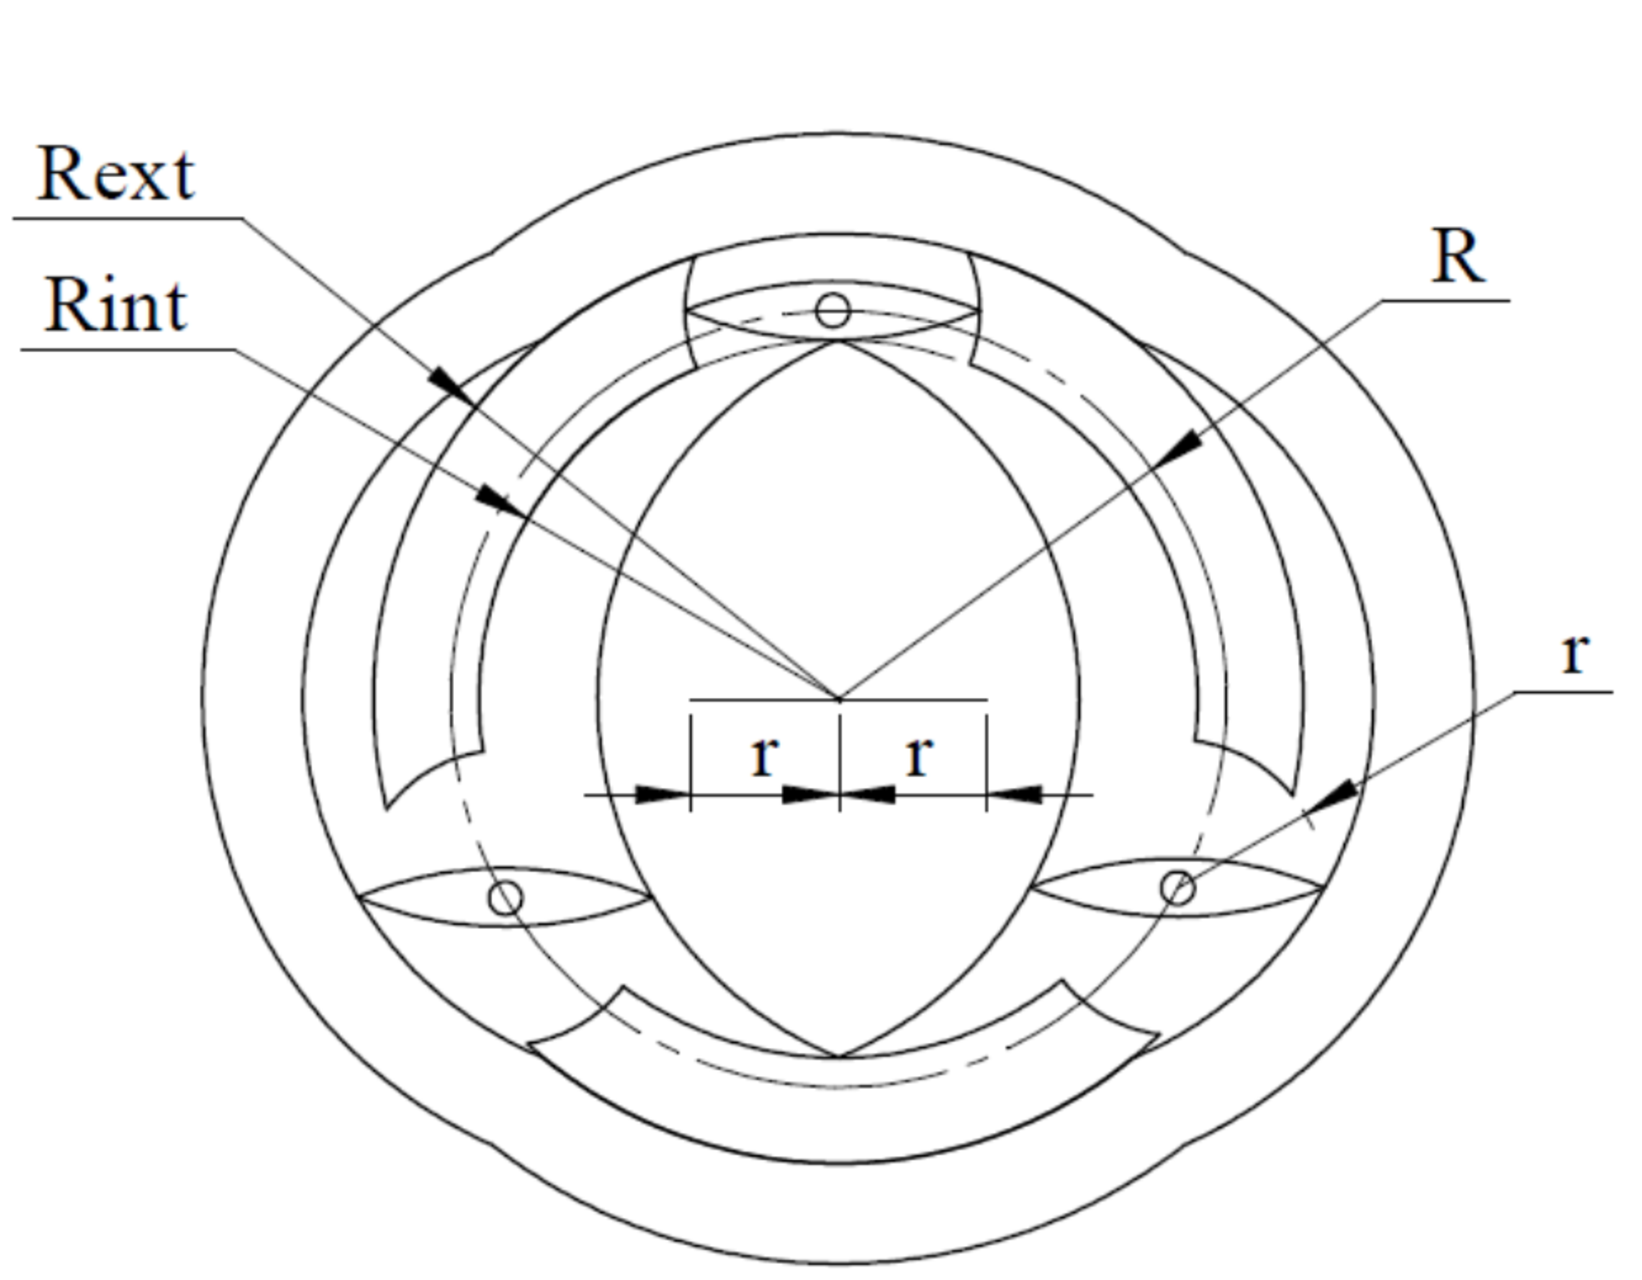
\includegraphics[width=\textwidth]{plano_mrcvc_flor.pdf}
  \caption{Parámetros goemétricos del MRCVC~\parencite{roldan}}\label{fig:geom_flor_mrcvc}
\end{figure}

\begin{figure}[ht]
  \centering
  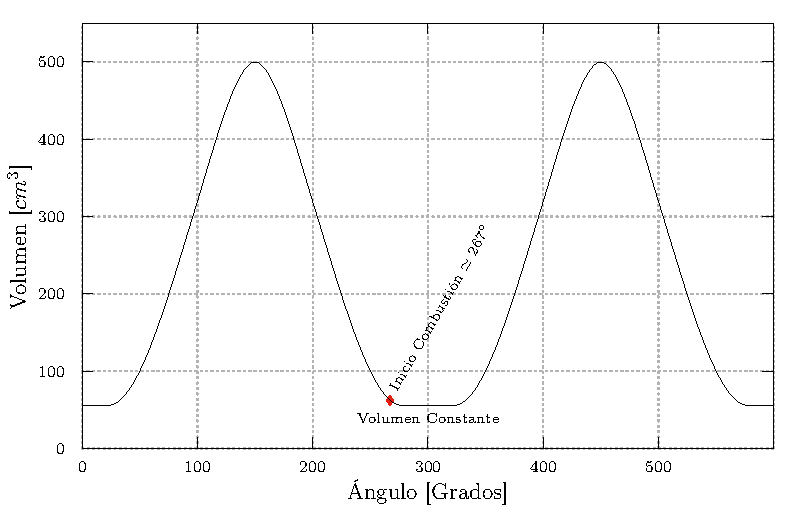
\includegraphics[width=\textwidth]{gnuplot/vol.pdf}
  \caption{Variación del volúmen del MRCVC}\label{fig:mrcvc_vol_cte}
\end{figure}

\begin{figure}[ht]
  \centering
  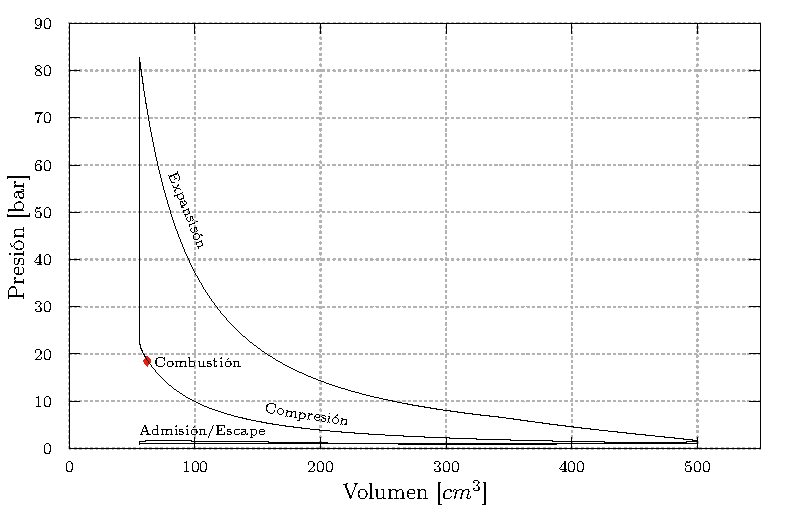
\includegraphics[width=\textwidth]{gnuplot/vol_vs_pres.pdf}
  \caption{Ciclo operativo del MRCVC}\label{fig:PV_mrcvc}
\end{figure}


El ciclo operativo ideal del MRCVC es considerado un ciclo Otto en el que las
carreras de admisión, compresión, expansión y escape ocurren a medida que el
fluido de trabajo rota con respecto al eje del cigüeñal.
%
En la Figura~\ref{fig:ciclo_mrcvc} se puede ver una progresiva del ciclo del
MRCVC con estas carreras representadas en AZUL para la admisión, compresión en
AMARILLO, expansión en ROJO y escape o barrido en VIOLETA.

Durante el ciclo se destaca un aspecto particular de este motor, siguiendo la
paleta de color negro se ve que durante el proceso de compresión y combustión,
las paletas que forman la frontera aguas arriba y aguas abajo de la cámara de
combustión cambian.
%
La paleta que delimita el frente de la cámara se retrasa con respecto a la
cámara con la que inició el ciclo, produciendo que este dure más de una
revolución resultando en  en $600^{\circ}$ de giro del cigüeñal para el caso de
3 paletas considerado en este trabajo.

Para un motor con las características geométricas indicadas en la
Tabla~\ref{tab:geom_mrcvc}, el volumen mínimo alcanzado permanece constante por
un período de $\sim 44,65^\circ$, como se puede ver en la
Figura~\ref{fig:mrcvc_vol_cte} en donde se representa la variación del volumen
con respecto al ciclo.
%
En este gráfico se indica el ángulo de inicio de la combustión, el cual \emph{es
una estimación} basada en datos de otros motores como
$\theta_{0}\simeq 267^{\circ}$.

\begin{figure}[ht]
  \centering
  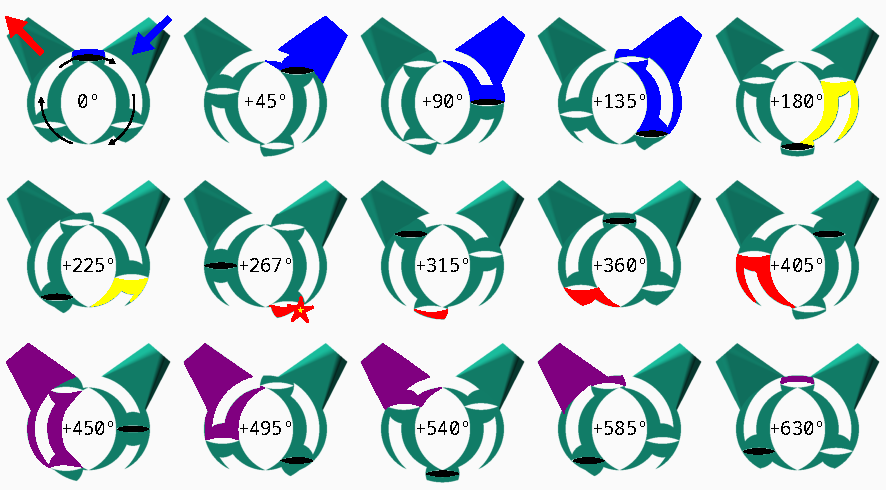
\includegraphics[width=\textwidth]{ciclo/ciclo_operativo.pdf}
  \caption{Ciclo operativo del MRCVC}\label{fig:ciclo_mrcvc}
\end{figure}

\begin{table}
    \centering
    \begin{tabular}{rccccccccc} \toprule
     Parámetro & n & R & r & $h_{c}$ & $h_{p}$ & rc & V0 & $R_i$ & $R_e$ \\ \midrule
     Valor & \lua{tex.print(myData.n)} & \lua{tex.print(myData.R)} & \lua{tex.print(myData.r)} & \lua{tex.print(myData.hc)} & \lua{tex.print(myData.hp)} & \lua{tex.print(myData.rc)} & \lua{tex.print(myData.V0)} & \lua{tex.print(trunc(myData.Ri))} & \lua{tex.print(trunc(myData.Re))} \\
     Unidades & --- & mm & mm & mm & mm & --- & $cm^3$ & mm & mm \\ \bottomrule
    \end{tabular}
    \caption{Geometría del MRCVC}\label{tab:geom_mrcvc}
\end{table}

\nomenclature[G]{\(R\)}{Radio de referencia del MRCVC, ver Figura \ref{fig:mrcvc_vol_cte}}
\nomenclature[G]{\(R_{i}\)}{Radio de cara interna del MRCVC, ver Figura \ref{fig:mrcvc_vol_cte}}
\nomenclature[G]{\(R_{e}\)}{Radio de cara externa del MRCVC, ver Figura \ref{fig:mrcvc_vol_cte}}
\nomenclature[G]{\(r\)}{Radio de trayectoria de paletas, ver Figura \ref{fig:mrcvc_vol_cte}}
\nomenclature[G]{\(n\)}{Número de paletas del MRCVC}
\nomenclature[G]{\(h_c\)}{Altura de cámara}
\nomenclature[G]{\(h_p\)}{Altura de puerto}

%%%%%%%%%%%%%%%%%%%%%%%%%%%%%%%%%%%%%%%%%%%%%%%%%%%%%%%%%%%%%%%%%%%%%%%%%%%%%%%

\subsection{Sistemas de Intercambio de Gases}
%
En un motor típico de combustión interna el sistema de intecambio de gases se
compone de una toma de aire, filtro, cuerpo de mariposa, puerto y conducto de
admisión, puerto y conducto de escape, catalizador y silenciador hasta
finalmente descargar en la atmósfera.

Para simplificar el sistema analizado no se tuvieron en cuenta elementos como:
mariposa, carburador, filtros de aire, convertidores catalíticos y demás; se
utilizó un sistema simplificado en el que solamente se tiene conducto de
admisión y escape junto con puertos de admisión y escape.
%
El eje de los conductos coincide con el eje del puerto, estos últimos hacen una
transición desde el diámetro del conducto hasta la altura de la ranura del
puerto en la cámara de combustión, en la
Figura~\ref{fig:sistema_intercambio_gases} se esquematiza la geometría
mencionada.

\begin{figure}
    \centering
    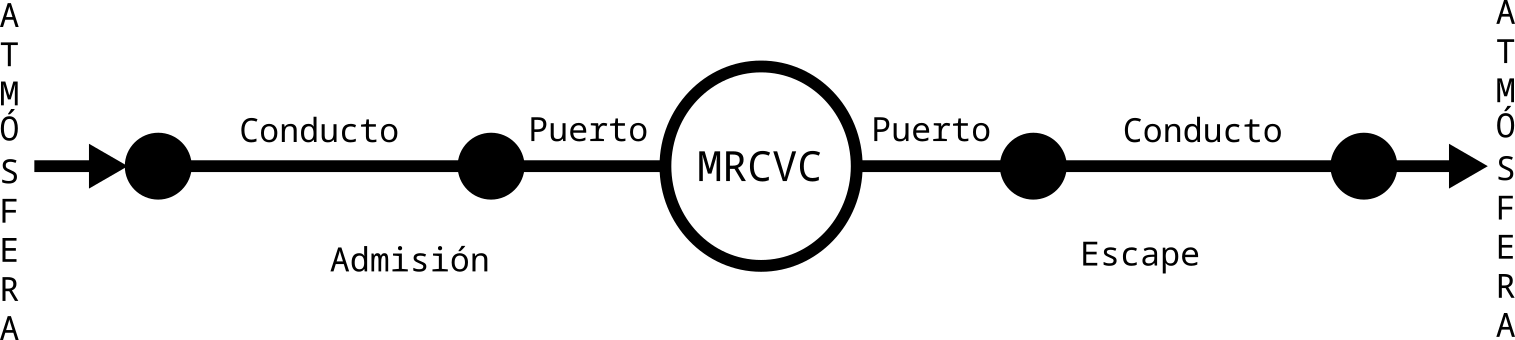
\includegraphics[width=\textwidth]{ciclo/sistema_intercambio_gases.png}
    \caption{Esquema del sistema de intercambio de gases}\label{fig:sistema_intercambio_gases}
\end{figure}


En trabajos anteriores~\parencite{lopez13} se demostró que se tiene una mejor
\emph{performance} del motor si se ubican los puertos en el cuerpo central, esto
comparado al rendimiento obtenido con los puertos ubicados en las tapas del
estator.
%
En dicho trabajo se realizó una optimización de la geometría mediante un barrido
paramétrico de las variables que determinan la forma, posición y reglaje de los
puertos, ya que es la ubicación angular de los puertos la que determina la
duración de los procesos de admisión y escape.
%
Los puertos están fijos en la periferia del estator y su posición se define con
los ángulos \emph{IIA}, \emph{IFA} para la admisión y \emph{EIA}, \emph{EFA}
para el escape, ver Figura~\ref{fig:angulos_puertos}.

\nomenclature[G]{\(IIA\)}{Ángulo de apertura del puerto de admisión, ver Figura \ref{fig:angulos_puertos}}
\nomenclature[G]{\(IFA\)}{Ángulo de cierre del puerto de admisión, ver Figura \ref{fig:angulos_puertos}}
\nomenclature[G]{\(EIA\)}{Ángulo de apertura del puerto de escape, ver Figura \ref{fig:angulos_puertos}}
\nomenclature[G]{\(EFA\)}{Ángulo de cierre del puerto de escape, ver Figura \ref{fig:angulos_puertos}}

\begin{figure}
    \centering
    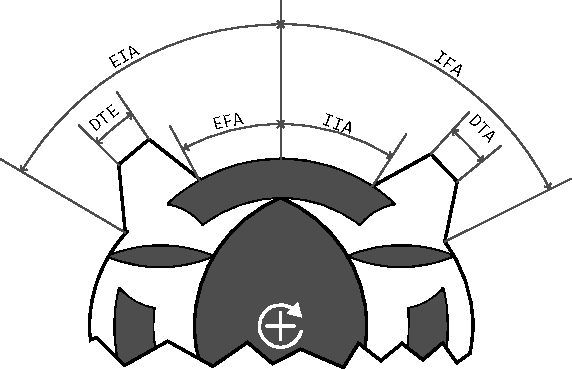
\includegraphics[width=0.8\textwidth]{/CAD/angulos.pdf}
    \caption{Puerto de admisión y escape}\label{fig:angulos_puertos}
\end{figure}
